The majority of physics analyses that employ ECAL timing focus on prompt signals, defined as energy deposits arising from particles produced at the primary vertex (PV) with no significant displacement in space or delay in time.
In contrast, delayed signals arise when a long-lived particle (LLP) travels a macroscopic distance from the PV before decaying, often with a velocity $\beta < 1$.
The decay products of such particles can therefore arrive at the ECAL with significantly delayed times relative to prompt particles.
Accurate reconstruction of large delay times is essential for analyses targeting LLP signatures.

The performance of the CC timing algorithm for delayed signals is studied using simulated samples containing LLP decays that produce sizable delays in the ECAL.
To quantify the accuracy of the reconstructed times, a reference generator-level time is required.
For each reconstructed hit (rechit), a generator-level time (\emph{gen-time}) is computed from the simulated energy deposits in the ECAL crystals, recorded as \texttt{pCaloHits}.
The gen-time of a rechit is defined as the energy-weighted average of the times of the \texttt{pCaloHits} contributing to the reconstructed pulse.

Figure~\ref{pc_v_cc_bais} shows the reconstructed rechit time obtained with the CC algorithm as a function of the corresponding gen-time.
No timing calibration is applied to the reconstructed times.
For delays exceeding approximately 1~ns, a systematic bias is observed, with the reconstructed time underestimating the true delay.
The right panel of Fig.~\ref{pc_v_cc_bais} shows an expanded view of the region below approximately 1~ns, where good agreement between the CC reconstruction and the gen-time is observed, indicating accurate performance for prompt and mildly delayed signals.

\begin{figure}[h!tbp]
\begin{center}
\resizebox{0.45\textwidth}{!}{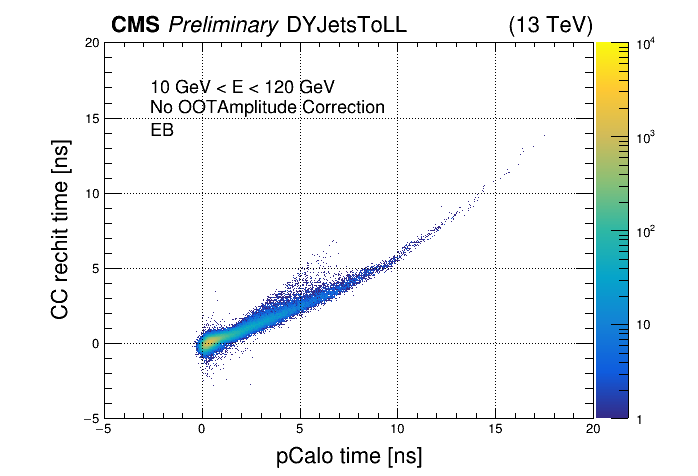
\includegraphics{fig/sec_gen/tr_2d_PCvCC_delay_13062022150058.png}}
\resizebox{0.45\textwidth}{!}{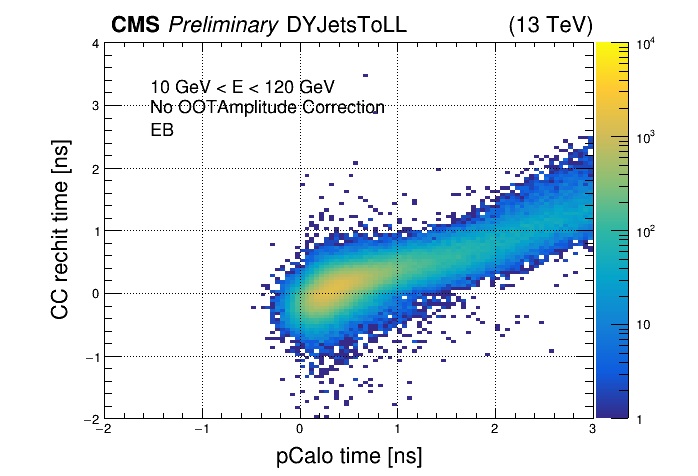
\includegraphics{fig/sec_gen/tr_2d_PCvCC_delay_zoom_13062022150920.png}}
\caption{Generator-level rechit time as a function of the rechit time reconstructed with the CC algorithm in simulated events containing delayed signals.
The reconstructed times are uncalibrated.
Left: a systematic bias is observed for delays greater than approximately 1~ns.
Right: an expanded view of the region below approximately 1~ns, where good agreement with the generator-level time is observed.}
\label{pc_v_cc_bais}
\end{center}
\end{figure}

To identify the origin of this bias, the CC timing reconstruction is repeated with the out-of-time (OOT) amplitude correction disabled.
Figure~\ref{pc_v_cc_nooot} shows the reconstructed rechit time obtained with this modified CC algorithm as a function of the gen-time.
In this configuration, no significant bias is observed at large delay times, demonstrating that the bias originates from the OOT amplitude correction step.

\begin{figure}[h!tbp]
\begin{center}
\resizebox{0.7\textwidth}{!}{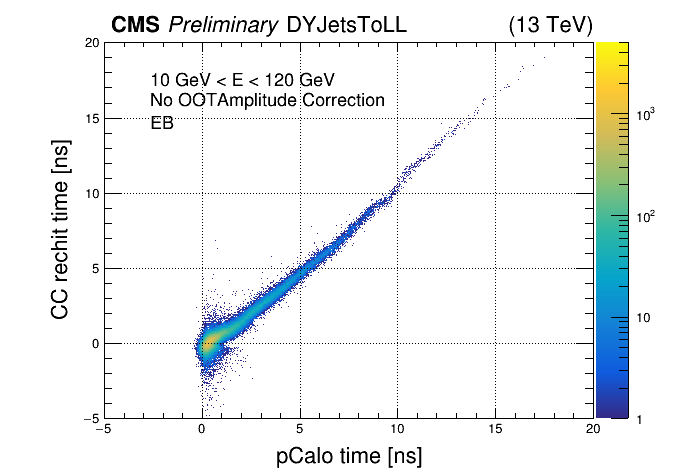
\includegraphics{fig/sec_gen/tr_2d_PCvCC_delay_nocorr_09062022175333.png}}
\caption{Generator-level rechit time as a function of the rechit time reconstructed with the CC algorithm when the OOT amplitude correction is disabled.
No significant bias is observed at large delay times.}
\label{pc_v_cc_nooot}
\end{center}
\end{figure}

As discussed in Section~\ref{sec:algo2}, the OOT amplitude correction relies on amplitudes returned by the multi-fit energy reconstruction, which assumes that out-of-time contributions occur at fixed time offsets corresponding to integer multiples of the LHC bunch spacing.
For delayed signals, this assumption is violated because the relative timing of pulse contributions varies continuously with the particle time of flight.
As a result, the fitted OOT amplitudes no longer accurately describe the true pulse composition, leading to a biased correction of the reconstructed pulse shape and, consequently, of the reconstructed time.

To accommodate analyses involving delayed signatures, the CC algorithm provides two reconstructed time quantities: one with and one without the OOT amplitude correction.
The corrected time, which benefits from mitigation of OOT pileup, is optimal for prompt physics analyses.
The uncorrected time, while exhibiting degraded resolution due to residual pileup contributions, remains unbiased at large delays and is therefore suitable for analyses targeting LLP signatures.
Both timing quantities are available in the ECAL reconstructed hit collection within the CMS software framework (CMSSW).
